\documentclass{fizykalab}

% Variables
\def\pomvspace{\vspace{0.3em}}

% Ustawienia strony
\usepackage{lipsum}
\usepackage[margin=3cm]{geometry}
\usepackage{graphicx}
\usepackage{enumitem}
\usepackage{siunitx}
\usepackage{amsmath}
\usepackage{cancel}
\usepackage{makecell}
\usepackage{mathtools}
\setlist{leftmargin=15pt,labelindent=15pt}
\setlist[enumerate]{noitemsep,wide=0pt, leftmargin=*}

% Ustawienia stopki
\usepackage{lastpage}
\usepackage{fancyhdr}
\pagestyle{fancy}
\fancyhf{} % sets both header and footer to nothing
\renewcommand{\headrulewidth}{0pt}
\cfoot{\thepage\ z \pageref{LastPage}}

% Ustawienia do tabelki
\wydzial{IEiT}
\autorjeden{Robert Mesek}
\autordwa{}
\rok{II}
\grupa{8 - L}
\zespol{6}
\temat{Ćwiczenie zerowe}
\nrcwiczenia{0}
\datawykonania{03.10.2023}
\dataoddaniajeden{}
\zwrotdopoprawy{}
\dataoddaniadwa{}
\datazaliczenia{}

\begin{document}

\maketitle

\section*{Układ pomiarowy i oznaczenia}
 {\setlength{\parindent}{0pt}

  \begin{figure}[htp]
	  \begin{minipage}[t]{0.5\textwidth}
		  \centering
		  \vspace{0pt}
		  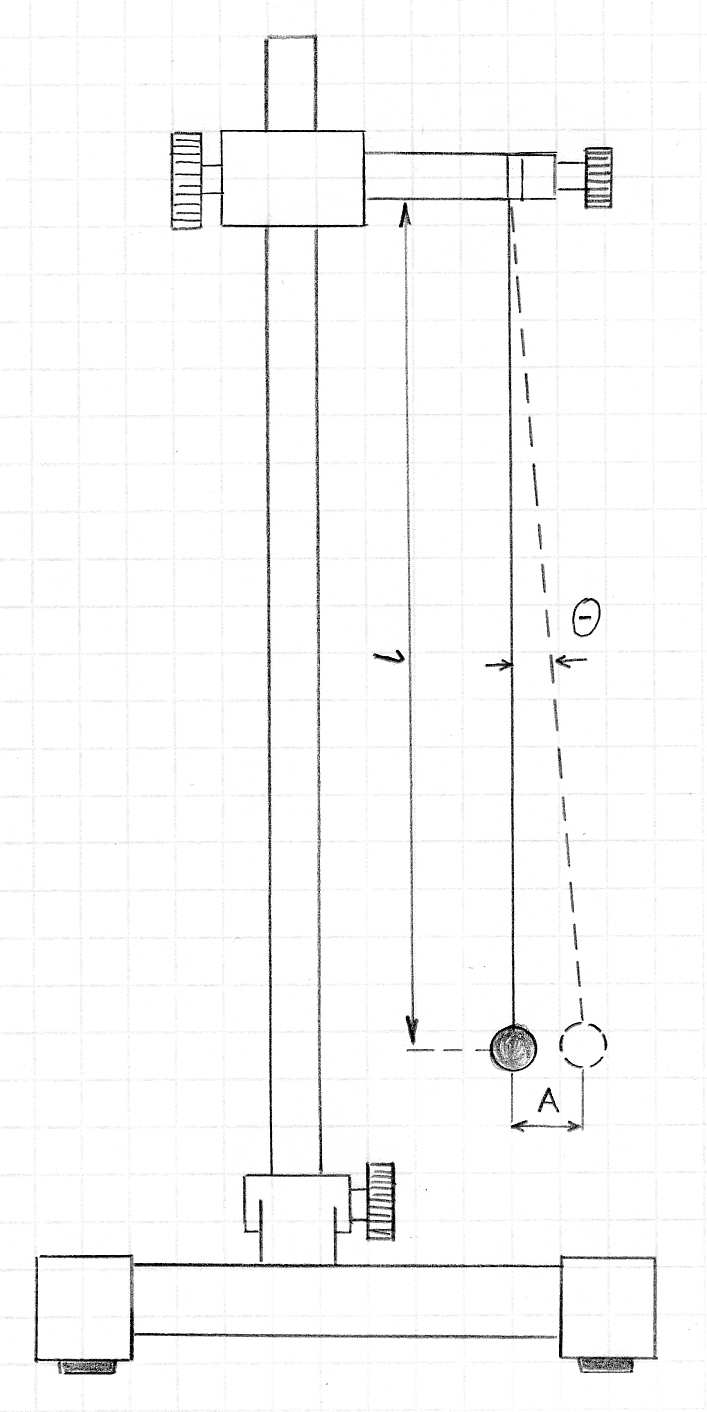
\includegraphics[width=0.8\linewidth]{images/zestaw-wahadla.png}
		  \caption{Zestaw Wahadła}
		  \label{fig:zestaw-wahadla}
	  \end{minipage}%
	  \hfill
	  \begin{minipage}[t]{0.5\textwidth}
		  \vspace{1em}

		  \begin{enumerate}


			  \item Zestaw wahadła prostego (Rys.~\ref{fig:zestaw-wahadla})

			  \item Sekundomierz (stoper) \\ dokładność \SI{1}{\second}

			  \item Przymiar milimetrowy (linijka) \\ dokładność \SI{1}{\milli\meter}

		  \end{enumerate}

		  $ t $ \quad czas

		  $ l $ \quad długość wahadła

		  $ \theta $ \quad kąt wychylenia od położenia równowagi

		  $ g $ \quad przyśpieszenie ziemskie

		  $ T $ \quad okres drgań

		  %$ u_l $ \quad niepewność maksymalna pomiaru długości wahadła

		  %$ u_t $ \quad niepewność maksymalna pomiaru czasu

		  %$ u_g $ \quad niepewność przyśpieszenia ziemskiego

	  \end{minipage}%
	  \hspace*{\fill}
  \end{figure}
 }


\newpage

\section*{Ćwiczenie ,,0'': Opracowanie danych pomiarowych}
 {\setlength{\parindent}{0pt}
  \paragraph{Cel ćwiczenia:}
  Zaznajomienie się z typowymi metodami opracowania danych pomiarowych przy wykorzystaniu wyników pomiarów dla wahadła prostego.
  \newline

  \par
  Wahadło proste jest, jak wskazuje jego nazwa, układem mechanicznym charakteryzującym się prostotą tak eksperymentu jak i opisu teoretycznego. Dlatego nadaje się dobrze na ćwiczenie wprowadzające (zerowe), mające na celu poznanie podstawowych metod opracowania danych pomiarowych. Interpretacja wyników opiera się na równaniu określającym okres drgań $T$ jako funkcję długości wahadła $l$ oraz przyspieszenia ziemskiego $g$,
  \[\boxed{T = 2 \pi \sqrt{ \frac{l}{g} }}\text{\space.}\tag{0}\]
  Wzór ten jest słuszny, jeśli wychylenie ciężarka z położenia równowagi jest małe.
 }

\section*{Przekształcenie wzoru}
 {\setlength{\parindent}{0pt}
  \[ T = 2 \pi \sqrt{ \frac{l}{g} } \]
  \[\Downarrow\]
  \[ T^2 = 4 \pi^2 \frac{l}{g} \]
  \[\Downarrow\]
  \begin{equation}
	  \boxed{
		  g = 4\pi^2\cdot\frac{l}{T^2}
	  }
	  \tag{1}
  \end{equation}
  Wykorzystamy ten wzór do obliczania przyśpieszenia ziemskiego.
 }

\section*{Niepewności pomiarowe}
 {\setlength{\parindent}{0pt}
  \par
  \textbf{Uwzględniamy niepewności wynikające z odczytu danych:}

  $\bullet$ pomiar długości: $\SI{2}{\milli\meter} = \SI{0.002}{\meter}$ (z rozsądku)

  $\bullet$ pomiar czasu: $\SI{30}{\milli\second} = \SI{0.03}{\second}$ (czas reakcji człowieka)
 }

\newpage

\section*{Sposób pierwszy}
 {\setlength{\parindent}{0pt}
  \subsection*{Wykonanie ćwiczenia}
  \par
  1. Mierzymy długość wahadła ($l$).

  2. Wykonujemy dziesięć pomiarów okresów dziesięciu okresów wahadła ($T$).

  3. Uwzględniamy błąd pomiarowy wynikający z dokładności sprzętu oraz błąd ludzki.

  4. Korzystając ze wzoru (1) obliczamy $g$.


  \subsection*{Wyniki pomiarów}
  \par
  Zmierzona długość wahadła \quad $l = \SI{520}{\milli\meter} = \SI{0.52}{\meter}$
  \pomvspace

  Najmniejsza działka przyrządu \quad $ \Delta l = \SI{1}{\milli\meter} = \SI{0.001}{\meter} $
  \pomvspace

  \begin{table}[!ht]
	  \centering
	  \begin{tabular}{|l | l | l | l|}
		  \hline
		  \rule{0pt}{4ex}\makecell{Numer                                                                                  \\ pomiaru} & \makecell{Czas 10 \\ okresów} & \makecell{Czas 1 \\ okresu} & \makecell{Kwadrat odchyłki \\ od średniej} \\ [0.5ex]
		  \hline\hline
		  \rule{0pt}{3ex}$i$ & $10 \ T_i[s]$ & $T_i[s]$               & $(T_i - T_\text{śr})^2[s^2]$                      \\
		  \hline
		  $1$                & $14.08$       & $1.408$                & $0.00190969$                                      \\
		  \hline
		  $2$                & $14.13$       & $1.413$                & $0.00149769$                                      \\
		  \hline
		  $3$                & $14.44$       & $1.444$                & $0.00005929$                                      \\
		  \hline
		  $4$                & $14.79$       & $1.479$                & $0.00074529$                                      \\
		  \hline
		  $5$                & $14.63$       & $1.463$                & $0.00012769$                                      \\
		  \hline
		  $6$                & $14.54$       & $1.454$                & $0.00000529$                                      \\
		  \hline
		  $7$                & $14.52$       & $1.452$                & $0.00000009$                                      \\
		  \hline
		  $8$                & $14.62$       & $1.462$                & $0.00010609$                                      \\
		  \hline
		  $9$                & $14.74$       & $1.474$                & $0.00049729$                                      \\
		  \hline
		  $10 = N$           & $14.68$       & $1.468$                & $0.00026569$                                      \\
		  \hline
		  \rule{0pt}{3ex}    &               & $T_\text{śr} = 1.4517$ & $\sum_{i=1}^{10}{(T_i - T_\text{śr})^2} = 0.0052$ \\ [0.5ex]
		  \hline
	  \end{tabular}
	  \caption*{Tabela 1}
  \end{table}

  \subsection*{Opracowanie wyników}
  \subsubsection*{Błędy grube}
  \par
  Po przeanalizowaniu wyników, nasze pomiary nie zawierają błędów grubych.

  $T_{\text{max}} = \SI{14.79}{\second}$ \quad $T_{\text{min}} = \SI{14.08}{\second}$ \quad $\Delta T = \SI{0.71}{\second}$

  \subsection*{Niepewność pomiaru typu A}
  \par
  Niepewność standardowa średniego okresu z pomiaru wielokrotnego
  \begin{gather*}
	  u_A(T_\text{śr}) = \sqrt{ \frac{ \sum{(T_i - T_\text{śr})^2} }{ N(N-1) } } = \sqrt{\frac{0.0052}{10*9}} \ [\sqrt{(\SI{}{\second})^2}] = \SI{0.0076}{\second}
  \end{gather*}

  \par
  Niepewność względna średniego okresu
  \[ \frac{u_A(T_\text{śr})}{T_\text{śr}} = \frac{\SI{0.0076}{\second}}{\SI{1.4517}{\second}} =  0.0052\]

  \subsection*{Niepewność pomiaru typu B}
  \par
  Niepewność pomiaru okresu
  \[ u_B(T) = \frac{\SI{30}{\milli\second}}{10} = \SI{3}{\milli\second}\ = \SI{0.003}{\second} \]

  \par
  Niepewność standardowa pomiaru długości
  \[ \frac{\Delta l}{\sqrt{3}} = \frac{1}{\sqrt{3}} \SI{}{\milli\meter} = \SI{0.577}{\milli\meter} = \SI{5.77e-4}{\meter} \]

  \par
  Niepewność maksymalna pomiaru długości
  \begin{align*}
	   & u_B(l) = \textit{niepewność pomiaru długości} + \frac{\Delta l}{\sqrt{3}}
	  \\
	   & u_B(l) = 2 + \frac{1}{\sqrt{3}}= 2.5774 \ [\SI{}{\milli\meter}] \approx \SI{0.0026}{\meter}
  \end{align*}

  \par
  Niepewność względna pomiaru długości wahadła
  \[ \frac{u_B(l)}{l} = \frac{ 2.5774\cancel{ \SI{}{\milli\meter}} }{ 520\cancel{ \SI{}{\milli\meter}} } = 0.0050\]

  \subsection*{Niepewność złożona}
  \par
  Niepewność złożona dla pomiarów okresu
  \[ u_c(T) = \sqrt{u_A^2(T) + u_B^2(T)} = \SI{0.0082}{\second}\]

  \par
  Niepewność złożona dla pomiaru długości
  \[ u_c(l) = \sqrt{u_A^2(l) + u_B^2(l)} = u_B(l) = \SI{0.0026}{\meter}\]

  \par
  Niepewność złożona $u_c(g)$ dla $l = \SI{0.52}{\meter}$ i $T = \SI{1.4517}{\second}$
  \begin{gather*}
	  u_c(g) = \sqrt{ \left( \frac{\partial g}{\partial l} u_c(l) \right)^2 + \left( \frac{\partial g}{\partial T} u_c(T) \right)^2 } = \sqrt{ \left( \frac{4\pi^2}{T^2} u_c(l) \right)^2 + \left( \frac{8\pi^2l}{T^3} u_c(T) \right)^2 } = 0.1203 \ \frac{\SI{}{\meter}}{\SI{}{\second}^2}
  \end{gather*}

 }

\subsection*{Niepewność rozszerzona}
\par
Zakładając, że współczynnik rozszerzenia wynosi $k_p = 2$, to niepewność rozszerzona $U$ wynosi
\[ U(g) = k_p \cdot u_c(g) = 0.2406 \ \frac{\SI{}{\meter}}{\SI{}{\second}^2} \]

\subsection*{Przyśpieszenie ziemskie}
\par
Obliczamy przyśpieszenie ziemskie
\[ g = 4\pi^2\cdot\frac{l}{T_\text{śr}^2} =  4\pi^2\cdot\frac{0.52}{(1.4517)^2} \approx 9.74 \ \frac{\SI{}{\meter}}{\SI{}{\second}^2} \]


\newpage


\section*{Sposób drugi}
 {\setlength{\parindent}{0pt}
  \subsection*{Wykonanie ćwiczenia}
  \par
  Wyznaczymy przyspieszenie ziemskie mierząc okresy drgań dla różnych długości wahadła.
  \[ T = 2\pi\sqrt{\frac{l}{g}} \]
  Przekształcamy ten wzór i zapisujemy jako zależność liniową
  \begin{equation}
	  \boxed{
		  T^2 = \frac{4\pi^2}{g}l
	  }
	  \tag{wzór roboczy}
  \end{equation}
  przy czym $T$ to okres drgań, $L$ to długość wahadła, zaś $g$ jest przyspieszeniem ziemskim.

  \pomvspace
  \par
  Zmierzymy długość wahadła oraz czas trwania 10 okresów. Następnie dla otrzymanych 4 punktów skorzystamy z regresji liniowej, aby znaleźć szukane parametry i ich niepewności.

  \subsection*{Wyniki pomiarów}
  \par
  \begin{table}[!ht]
	  \centering
	  \begin{tabular}{|l|l|l|l|l|l|}
		  \hline
		  % HEADER
		  \makecell{Numer                                                                                                         \\ pomiaru} & \makecell{Długość \\ wahadła} & \makecell{Czas 10 \\ okresów} & \makecell{Czas 1 \\ okresu} & \makecell{Kwadrat \\ okresu}  \\ \hline\hline
		  % END HEADER
		  \rule{0pt}{3ex}$i$ & $l_i[\SI{}{\meter}]$ & $10T_i[\SI{}{\second}]$ & $T_i[\SI{}{\second}]$ & $10T_i^2[\SI{}{\second}]$ \\ \hline

		  $1$                & $0.106$              & $6.15$                  & $0.615$               & $0.3782$                  \\ \hline
		  $2$                & $0.150$              & $7.48$                  & $0.748$               & $0.5595$                  \\ \hline
		  $3$                & $0.197$              & $8.63$                  & $0.863$               & $0.7447$                  \\ \hline
		  $4$                & $0.238$              & $9.43$                  & $0.943$               & $0.8892$                  \\ \hline
		  $5$                & $0.282$              & $10.36$                 & $1.036$               & $1.0732$                  \\ \hline
		  $6$                & $0.322$              & $11.00$                 & $1.100$               & $1.2100$                  \\ \hline
	  \end{tabular}
	  \caption*{Tabela 2}
  \end{table}

  \subsection*{Opracowanie wyników}
  \par
  Zlinearyzowany wzór $T^2(l) = \frac{4\pi^2}{g}l$ i dane z tabeli (Tabela 2) wykorzystujemy do obliczenia współczynników prostej przyjmując:

  \quad $y$ za $T^2$

  \quad $x$ za $l$

  \quad współczynnik kierunkowy $a$ za $\frac{4\pi^2}{g}$

  danej równaniem $y = ax$, aby oszacować przyspieszenie ziemskie $g$.

  \par
  Wykorzystując funkcję \textbf{LINEST()} programu \textbf{Excel} otrzymaliśmy
  \[ a = 3.7966 \ \frac{\SI{}{\second}^2}{\SI{}{\meter}} \quad\quad u(a) = -0.0088 \ \frac{\SI{}{\second}^2}{\SI{}{\meter}}\]
  \[ u(g) = \sqrt{\left( \frac{dg}{da}u(a) \right)^2} = \left| \frac{dg}{da}u(a) \right| = \left| -\frac{4\pi^2}{a^2}u(a) \right| \approx 0.03 \ \frac{\SI{}{\meter}}{\SI{}{\second}^2}\]

  \begin{equation*}
	  \boxed{
		  a = \frac{4\pi^2}{g} \Leftrightarrow g = \frac{4\pi^2}{a} = \frac{4\pi^2}{3.7966} \approx 10.40 \ \frac{\SI{}{\meter}}{\SI{}{\second}^2}
	  }
  \end{equation*}


  \newpage

  \subsection*{Wykresy}
  \par
  \begin{figure}[!ht]
	  \caption*{Wykres zależności okresu drgań $T$ od długości wahadła $l$}
	  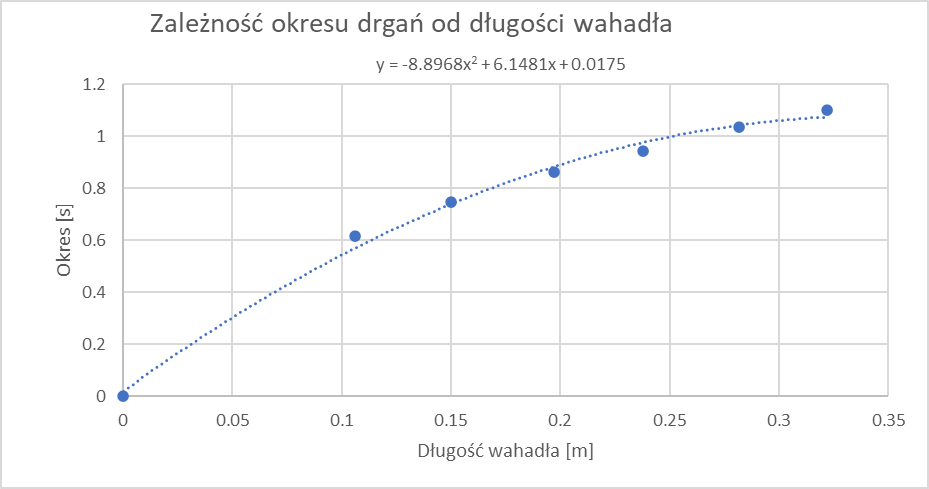
\includegraphics[width=1\linewidth]{images/okres-dlugosc.png}
	  \centering
  \end{figure}

  \par
  \begin{figure}[!ht]
	  \caption*{Wykres zależności kwadratu okresu drgań $T^2$ od długości wahadła $l$}
	  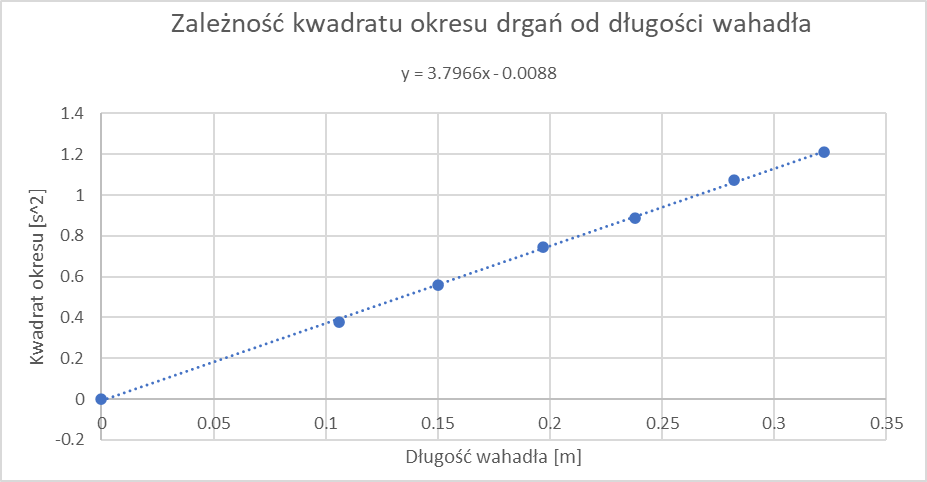
\includegraphics[width=1\linewidth]{images/okres_kwadrat-dlugosc.png}
	  \centering
  \end{figure}

 }

\newpage

\section*{Wnioski}
 {\setlength{\parindent}{0pt}
  \par
  Dla sposobu pierwszego uzyskane wyniki są zgodne ze stałą przyspieszenia dla Krakowa $g = 9.81 \ \frac{\SI{}{\meter}}{\SI{}{\second}^2}$. Otrzymany wynik w tym prostym doświadczeniu jest relatywnie bliski wartości oczekiwanej, a niedokładności najprawdopodobniej zależą od czynników ludzkich. Aby uzyskać należałoby znaleźć bardziej dokładny sposób obsługi przyrządów pomiarowych.

  \par\mbox{}\newline
  Dla sposobu drugiego otrzymane przyspieszenie $g = 10.40 \ \frac{\SI{}{\meter}}{\SI{}{\second}^2}$ znacząco odbiega od oczekiwanej wartości. Najprawdopodobniej jest to skutek niedokładności pomiarowych spowodowane czynnikiem ludzkim oraz także, wzór z którego korzystaliśmy (0) jest bliższy prawdziwych wartości okresu wahadła dla małych kątów wychylenia $\theta$, a w pomiarach $l_1$ i $l_2$ (Tabela 2) długość wahadła mogła być za krótka.

 }

%\section*{Bibliografia}
% {\setlength{\parindent}{0pt}
%
% }

\end{document}
